\documentclass[8pt,a4paper,compress]{beamer}

\usepackage{/home/siyer/lib/slides}

\title{What is Computer Science?}
\date{}

\begin{document}
\begin{frame}
\vfill
\titlepage
\end{frame}

\begin{frame}
\frametitle{Outline}
\tableofcontents
\end{frame}

\section{What is Computer Science?}
\begin{frame}[fragile]
\pause

Computer science is the study of automating processes that scale

\pause
\bigskip

A computer scientist is someone who specializes in the theory of computation and the design of computational systems

\pause
\bigskip

Important concepts at the heart of computer science
\begin{itemize}
\item Data
\item Algorithms
\item Programming
\item Abstraction
\end{itemize}
\end{frame}

\section{Data}
\begin{frame}[fragile]
\pause

We live in an era of data overload

\pause
\bigskip

For example
\begin{itemize}
\item Google, when searched for ``Alan Turing'', finds approximately 500 thousand pages, ranked in order of estimated relevance and usefulness 
\item Facebook has approximately 1.7 billion active users generating billions of comments and ``Likes'' each day 
\item GenBank, a national database of DNA sequences, has over 1 billion entries 
\item The Large Hadron Collider (LHC) at CERN produces collision data at the rate of 25 petabytes ($1 \text{petabyte} = 10^{15}$ bytes) per year
\end{itemize}

\pause
\bigskip

All these data would be junk without ideas and tools from computer science
\end{frame}

\section{Algorithms}
\begin{frame}[fragile]
\pause

An algorithm is a precise sequence of steps for carrying out a task, such as ranking web pages in Google, or finding closely related genes in GenBank

\pause
\bigskip


\begin{minipage}{200pt}
Example of an algorithm to estimate $\pi$

\begin{enumerate}
\item Draw a square that is 2 by 2 feet
\item Inscribe a circle of radius 1 foot (diameter 2 feet) inside the square
\item Grab a bucket of $n$ darts, move away from the dartboard, and put on a blindfold
\item Throw each dart randomly (but assume that your throwing skills ensure that it will land somewhere on the square dartboard)
\item Record whether or not the dart landed inside the circle
\item When you have thrown all $n$ darts, divide the number that landed inside the circle by $n$ and multiply by 4 to obtain your estimate for $\pi$
\end{enumerate}
\end{minipage}%
\hfill
\begin{minipage}{100pt}
\begin{center}
\visible<3->{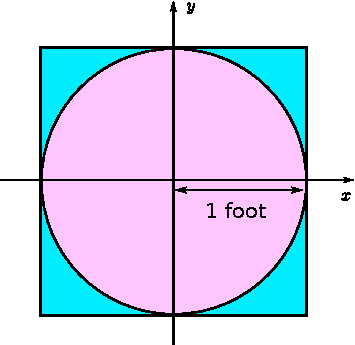
\includegraphics[scale=0.6]{figures/pi.pdf}}
\end{center}
\end{minipage}
\end{frame}

\section{Programming}
\begin{frame}[fragile]
\pause

A program is a list of instructions used to control the behavior of a computer

\pause
\bigskip

A programming language is a formal language designed to communicate those instructions to the computer

\pause
\bigskip

Types of programming languages
\begin{itemize}
\item Machine languages -- interpreted directly in hardware
\item Assembly languages -- thin wrappers over corresponding machine languages
\item High-level languages -- machine independent
\item System languages -- designed for writing low-level tasks, like memory and process management
\item Scripting languages -- generally extremely high-level and powerful
\item Domain-specific languages -- used in highly special-purpose areas only
\item Visual languages -- non-text based
\item Esoteric languages -- mostly of academic interest
\end{itemize}

\pause
\bigskip

In this course, you will learn three languages: PicoBot (domain-specific), HMMM (assembly), and Python (scripting)
\end{frame}

\section{Abstraction}
\begin{frame}[fragile]
\pause

Abstraction is the idea that when designing one part of a system, we can ignore the inessential details of other parts, provided we have a high-level understanding of what they do

\pause
\bigskip

In the design of software systems, abstraction ensures that many people can contribute to a project without everyone needing to understand everything
\end{frame}
\end{document}
